% Copyright 2004 by Till Tantau <tantau@users.sourceforge.net>.
%
% In principle, this file can be redistributed and/or modified under
% the terms of the GNU Public License, version 2.
%
% However, this file is supposed to be a template to be modified
% for your own needs. For this reason, if you use this file as a
% template and not specifically distribute it as part of a another
% package/program, I grant the extra permission to freely copy and
% modify this file as you see fit and even to delete this copyright
% notice. 

\documentclass{beamer}

% There are many different themes available for Beamer. A comprehensive
% list with examples is given here:
% http://deic.uab.es/~iblanes/beamer_gallery/index_by_theme.html
% You can uncomment the themes below if you would like to use a different
% one:
%\usetheme{AnnArbor}
%\usetheme{Antibes}
%\usetheme{Bergen}
%\usetheme{Berkeley}
%\usetheme{Berlin}
%\usetheme{Boadilla}
%\usetheme{boxes}
%\usetheme{CambridgeUS}
%\usetheme{Copenhagen}
%\usetheme{Darmstadt}
%\usetheme{default}
%\usetheme{Frankfurt}
%\usetheme{Goettingen}
%\usetheme{Hannover}
%\usetheme{Ilmenau}
%\usetheme{JuanLesPins}
%\usetheme{Luebeck}
\usetheme{Madrid}
%\usetheme{Malmoe}
%\usetheme{Marburg}
%\usetheme{Montpellier}
%\usetheme{PaloAlto}
%\usetheme{Pittsburgh}
%\usetheme{Rochester}
%\usetheme{Singapore}
%\usetheme{Szeged}
%\usetheme{Warsaw}
\usepackage{color}
\usepackage{graphicx}
\usepackage{subcaption}
\usepackage{hyperref}
\hypersetup{
    colorlinks=true,
    linkcolor=white,
    filecolor=magenta,      
    urlcolor=cyan,
}


\setbeamersize{text margin left=1mm,text margin right=1mm} 

\title{ATLAS Tile Calorimeter}

% A subtitle is optional and this may be deleted
\subtitle{TileCal Calib, DQ, DP, Performance and Processing meeting}

\author{Attila R\'adl\inst{1} \and Pratyush Anand\inst{2}

 }

% - Give the names in the same order as the appear in the paper.
% - Use the \inst{?} command only if the authors have different
%   affiliation.

\institute[] % (optional, but mostly needed)
{
  \inst{1}%
  Institute of Physics\\
  E\"otv\"os Lor\'and University
  
  \and
  \inst{2}%
  Department of Physics\\
  Indian Institute of Technology Madras
  
  \and
  \inst{3}%
  ATLAS TileCal Group\\
  CERN}
% - Use the \inst command only if there are several affiliations.
% - Keep it simple, no one is interested in your street address.

\date{\\\\$16^{th}$ July 2018}
% - Either use conference name or its abbreviation.
% - Not really informative to the audience, more for people (including
%   yourself) who are reading the slides online

\subject{Theoretical Computer Science}
% This is only inserted into the PDF information catalog. Can be left
% out. 

% If you have a file called "university-logo-filename.xxx", where xxx
% is a graphic format that can be processed by latex or pdflatex,
% resp., then you can add a logo as follows:

%\pgfdeclareimage[height=0.5cm]{university-logo}{university-logo-filename}
%\logo{\pgfuseimage{university-logo}}

\titlegraphic{
  \begin{picture}(0,0)
    \put(160,90){\makebox(0,0)[rt]{\includegraphics[width=3cm]{Cern.jpg}}}
  \end{picture}
  \begin{picture}(0,0)
    \put(-90,90){\makebox(0,0)[rt]{\includegraphics[width=3cm]{ATLAS-Logo-Ref-RGB-H_0.jpg}}}
  \end{picture}
 }

% Delete this, if you do not want the table of contents to pop up at
% the beginning of each subsection:

% Let's get started
\begin{document}

\begin{frame}
  \titlepage
\end{frame}

    
\begin{frame}{Introduction}
\textbf{Laser Data} : We use	the	laser calibration data produced by \textbf{Giulia di Gregorio} for 1/3 of the laser runs	since 2015 untill the end of 2017. She used the combined method to calculate the corrections (the	same method	used for this years corrections).\\	
\begin{center} \color{red}Thanks, Giulia! \end{center}\\
\textbf{Goals :}
\begin{itemize}
    \item study the average drift of the different cell types
    \item study the RMS of the variations in the channels (as done with Cesium)
    \item study on the difference between the measurements of the two PMTs connected to a given cell. 
\end{itemize}	\\\\	
NB:	The version used by Giulia is outdated (new developments by Henric not yet included). We will update this to the latest version of the calculation.\\
\textbf{Masked channels} : We exclude all channels that	are	masked in the HG (combined method uses HG).	
We also	exclude	those channels flagged as “affected” for the laser system. Non-instrumented	channels are also not used.	
  % You might wish to add the option [pausesections]
\end{frame}

% Section and subsections will appear in the presentation overview
% and table of contents.
\section{First Main Section}

\subsection{First Subsection}
\centering
\begin{frame}{Cesium Scans in Run 2}{}
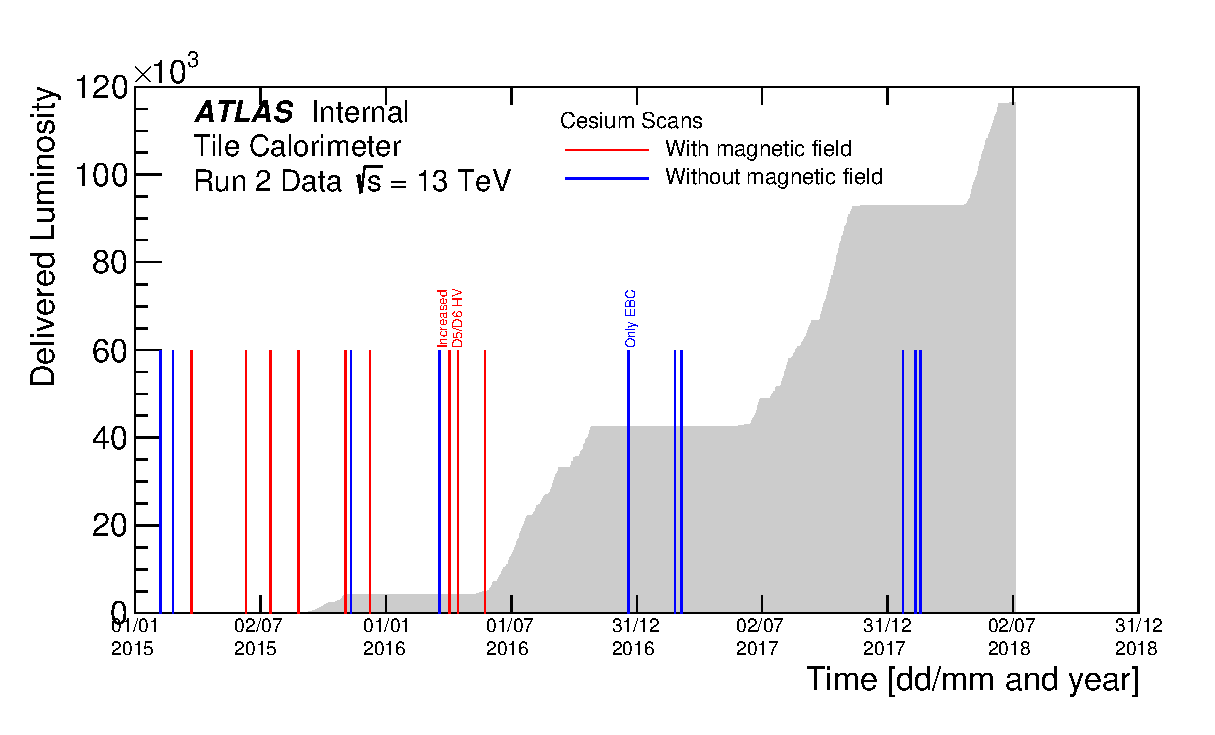
\includegraphics[width=0.9\textwidth]{CesiumScans_run2.eps}\\
Plan: Compare the drifts measured by Cesium	and	laser system during	several time periods (“IOV”), according	to Cesium scan availability.
\end{frame}

\subsection{Second Subsection}

% You can reveal the parts of a slide one at a time
% with the \pause command:
\begin{frame}{Cesium Vs Laser}
 \centering
 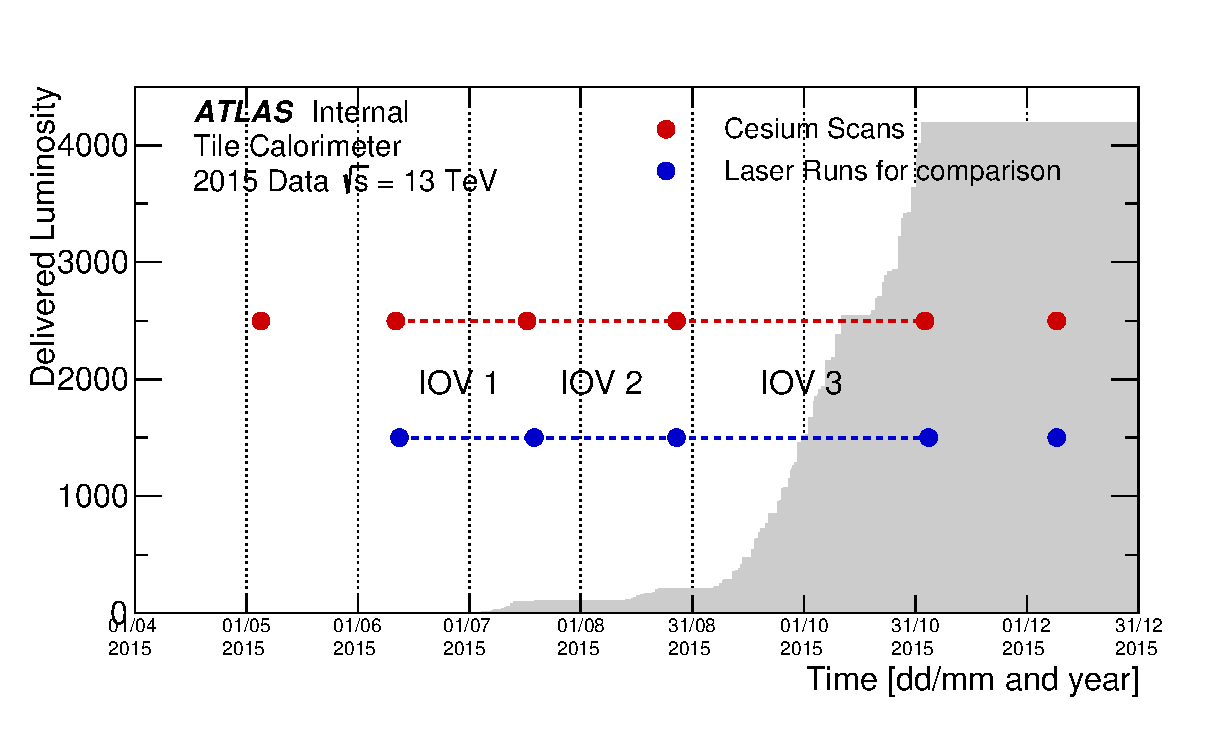
\includegraphics[width=\textwidth]{CsLas_IOVs_2015.eps}
 	\end{frame}
\subsection{Third Subsection} 	
\begin{frame}{Cesium Vs Laser}
 \begin{itemize}
     \item  We	start doing	a comparison in	2015, where	more scans were	performed.
     \item   We	defined	3 IOVs covering	different data taking periods. Laser runs selected	within 1 day of the	Cesium	scan \textbf{(avoided runs right after the scan)}.
    \item Cesium data: \textbf{Extracted Cesium	constants from COOL	DB}.
    \item Laser	data: Combined method using	\textbf{latest version of the code (new	smoothing)}.
    \item CESIUM (from DB, all with magnetic field)	
    \\IOV1:	263962 (11/june) $\leftrightarrow$ 270000 (17/july)
    \\IOV2:	270000 (17/july) $\leftrightarrow$ 277321 (27/aug)
    \\IOV3:	277321 (27/aug) $\leftrightarrow$ 284600 (3/nov)
    \item LASER	(new combined method, reference	from Giulia)
    \\IOV1:	267534 (12/june) $\leftrightarrow$ 272493 (19/july)
    \\IOV2:	272493 (19/july) $\leftrightarrow$ 277320 (17/aug	before	Cs)	
    \\IOV3:	277320 (17/aug) $\leftrightarrow$ 284682 (4/nov)
 \end{itemize}
	
\end{frame}
\section{Second Main Section}

\subsection{Another Subsection}
\begin{frame}{Part I}
\begin{center}\color{red}\Huge{Laser Study}\end{center}
\end{frame}
\begin{frame}{Laser runs in 2015}{}

\begin{figure}
\centering
\includegraphics[width=\textwidth]{drm15.pdf}
\caption{Average Drift vs Time}
\end{figure}
\end{frame}

\begin{frame}{Laser runs in 2015}{}
\begin{figure}
\centering
\includegraphics[width=0.9\textwidth]{drr151.pdf}
\caption{RMS of the Drift vs Time}
\end{figure}
NOTE : We will try to understand the jumps encircled above.
\end{frame}

\begin{frame}{Laser runs in 2015}{}
\begin{figure}
\centering
\includegraphics[width=\textwidth]{pmtm15.pdf}
\caption{$\Delta$PMT vs Time}
\end{figure}
\end{frame}

\begin{frame}{Laser runs in 2015}{}
\begin{figure}
\centering
\includegraphics[width=\textwidth]{pmtr15.pdf}
\caption{RMS of $\Delta$PMT vs Time}
\end{figure}
\end{frame}

\begin{frame}{Laser runs in 2015}{}
\begin{figure}
\centering
\includegraphics[width=\textwidth]{drm3.pdf}
\caption{Average Drift vs $\eta$ (Dec 12, 2015)}
\end{figure}
\end{frame}

\begin{frame}{Laser runs in 2015}{}
\begin{figure}
\centering
\includegraphics[width=0.9\textwidth]{drr3.pdf}
\caption{RMS of Drift vs $\eta$ (Dec 12, 2015)}
\end{figure}
NOTE : We will check the cells with large fluctuations.
\end{frame}

\begin{frame}{1-D Distributions for Laser runs in 2015}
\begin{figure}[H]
\centering
\begin{subfigure} [t] {0.49\textwidth}
\includegraphics[width=\textwidth]{LB1.pdf}
\caption{Long Barrel}
\end{subfigure}
\begin{subfigure} [t] {0.49\textwidth}
\includegraphics[width=\textwidth]{EB1.pdf}
\caption{Extended Barrel}
\end{subfigure}
\caption{Distribution of Drift (May 20, 2015)}
\end{figure}
\end{frame}



\begin{frame}{1-D Distributions for Laser runs in 2015}
\begin{figure}[H]
\centering
\begin{subfigure} [t] {0.49\textwidth}
\includegraphics[width=\textwidth]{LB3.pdf}
\caption{Long Barrel}
\end{subfigure}
\begin{subfigure} [t] {0.49\textwidth}
\includegraphics[width=\textwidth]{EB3.pdf}
\caption{Extended Barrel}
\end{subfigure}
\caption{Distribution of Drift (Dec 12, 2015)}
\end{figure}
\end{frame}

\begin{frame}{1-D Distributions for Laser runs in 2015}
\begin{figure}[H]
\centering
\begin{subfigure} [t] {0.49\textwidth}
\includegraphics[width=\textwidth]{pmtLB1.pdf}
\caption{Long Barrel}
\end{subfigure}
\begin{subfigure} [t] {0.49\textwidth}
\includegraphics[width=\textwidth]{pmtEB1.pdf}
\caption{Extended Barrel}
\end{subfigure}
\caption{Distribution of $\Delta$PMT (May 20, 2015)}
\end{figure}
NOTE : We will try to understand the peak at zero in D-cells in Long barrel.
\end{frame}



\begin{frame}{1-D Distributions for Laser runs in 2015}
\begin{figure}[H]
\centering
\begin{subfigure} [t] {0.49\textwidth}
\includegraphics[width=\textwidth]{pmtLB3.pdf}
\caption{Long Barrel}
\end{subfigure}
\begin{subfigure} [t] {0.49\textwidth}
\includegraphics[width=\textwidth]{pmtEB3.pdf}
\caption{Extended Barrel}
\end{subfigure}
\caption{Distribution of $\Delta$PMT (Dec 12, 2015)}
\end{figure}
\end{frame}


\begin{frame}{Laser runs in 2016}{}
\begin{figure}
\centering
\includegraphics[width=0.65\textwidth]{drm16.pdf}
\caption{Average Drift vs Time}
\end{figure}
\begin{itemize}
    \item We see jump of the D-cells since the HV was increased for D5 and D6 here.
    \item Giulia used a single reference (in 2015) for these points too. We'll update to a new reference each year.
\end{itemize}
\end{frame}
 

\begin{frame}{Laser runs in 2016}{}
\begin{figure}
\centering
\includegraphics[width=0.8\textwidth]{drr16.pdf}
\caption{RMS of the Drift vs Time}
\end{figure}
NOTE : We see jump of the D-cells since the HV was increased for D5 and D6 here.

\end{frame}

\begin{frame}{Laser runs in 2016}{}
\begin{figure}
\centering
\includegraphics[width=\textwidth]{pmtm16.pdf}
\caption{$\Delta$PMT vs Time}
\end{figure}
\end{frame}

\begin{frame}{Laser runs in 2016}{}
\begin{figure}
\centering
\includegraphics[width=\textwidth]{pmtr16.pdf}
\caption{RMS of $\Delta$PMT vs Time}
\end{figure}
\end{frame}

\begin{frame}{Laser runs in 2017}{}
\begin{figure}
\centering
\includegraphics[width=0.65\textwidth]{drm17.pdf}
\caption{Average Drift vs Time}
\end{figure}
\begin{itemize}
    \item We see jump of the D-cells since the HV was increased for D5 and D6 here.
    \item Giulia used a single reference (in 2015) for these points too. We'll update to a new reference each year.
\end{itemize}
\end{frame}

\begin{frame}{Laser runs in 2017}{}
\begin{figure}
\centering
\includegraphics[width=0.8\textwidth]{drr17.pdf}
\caption{RMS of the Drift vs Time}
\end{figure}
NOTE : We see jump of the D-cells since the HV was increased for D5 and D6 here.

\end{frame}

\begin{frame}{Laser runs in 2017}{}
\begin{figure}
\centering
\includegraphics[width=\textwidth]{pmtm17.pdf}
\caption{$\Delta$PMT vs Time}
\end{figure}
\end{frame}

\begin{frame}{Laser runs in 2017}{}
\begin{figure}
\centering
\includegraphics[width=\textwidth]{pmtr17.pdf}
\caption{RMS of $\Delta$PMT vs Time}
\end{figure}
\end{frame}



%Cs plots
\begin{frame}{Part II}
\begin{center}\color{red}\Huge{Comparison against Cesium}\end{center}
\end{frame}

\begin{frame}{Reminding about the IOV's}
 \centering
 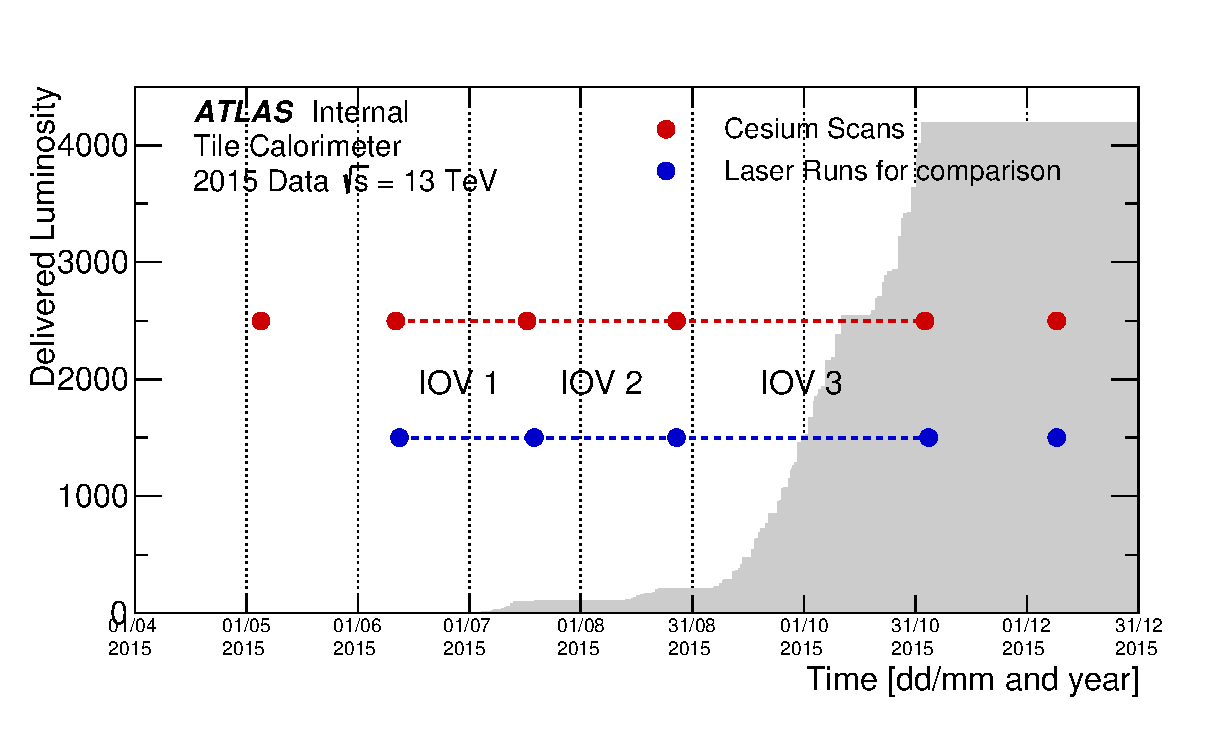
\includegraphics[width=\textwidth]{CsLas_IOVs_2015.eps}
 	\end{frame}


\begin{frame}{Laser vs Cesium Scans in 2015}
    \begin{figure}[H]
\centering
\begin{subfigure} [t] {0.3\textwidth}
\includegraphics[width=\textwidth]{colz_iov1.pdf}
\caption{IOV 1}
\end{subfigure}
\begin{subfigure} [t] {0.3\textwidth}
\includegraphics[width=\textwidth]{colz_iov2.pdf}
\caption{IOV 2}
\end{subfigure}
\begin{subfigure} [t] {0.3\textwidth}
\includegraphics[width=\textwidth]{colz_iov3.pdf}
\caption{IOV 3}
\end{subfigure}
\caption{Laser vs Cesium drift for all instrumented channels}
\end{figure}
\end{frame}

\begin{frame}{Laser vs Cesium Scans in 2015}
    \begin{figure}[H]
\centering
\begin{subfigure} [t] {0.3\textwidth}
\includegraphics[width=\textwidth]{colz_iov1.pdf}
\caption{IOV 1}
\end{subfigure}
\begin{subfigure} [t] {0.3\textwidth}
\includegraphics[width=\textwidth]{colz_iov2.pdf}
\caption{IOV 2}
\end{subfigure}
\begin{subfigure} [t] {0.3\textwidth}
\includegraphics[width=\textwidth]{colz_iov3.pdf}
\caption{IOV 3}
\end{subfigure}
\caption{Laser vs Cesium drift for all instrumented channels}
\end{figure}
\end{frame}



\begin{frame}{Laser vs Cesium Scans in 2015}
\begin{figure}[H]
\centering
\begin{subfigure} [t] {0.3\textwidth}
\includegraphics[width=\textwidth]{scatter_all_iov1.pdf}
\caption{IOV 1}
\end{subfigure}
\begin{subfigure} [t] {0.3\textwidth}
\includegraphics[width=\textwidth]{scatter_all_iov2.pdf}
\caption{IOV 2}
\end{subfigure}
\begin{subfigure} [t] {0.3\textwidth}
\includegraphics[width=\textwidth]{scatter_all_iov3.pdf}
\caption{IOV 3}
\end{subfigure}
\caption{Laser vs Cesium drift for different types of channels}
\end{figure}
\end{frame}

\begin{frame}{Laser vs Cesium Scans in 2015}
\begin{figure}[H]
\centering
\begin{subfigure} [t] {0.49\textwidth}
\includegraphics[width=\textwidth]{cs1d_a_lb_iov1.pdf}
\caption{Long Barrel}
\end{subfigure}
\begin{subfigure} [t] {0.49\textwidth}
\includegraphics[width=\textwidth]{cs1d_a_eb_iov1.pdf}
\caption{Extended Barrel}
\end{subfigure}
\caption{Laser and Cesium gain variation for A channels IOV 1}
\end{figure}
NOTE : We are investigating which channels return a zero variation in the cesium drift for these IOV's.

\end{frame}

\begin{frame}{Laser vs Cesium Scans in 2015}
\begin{figure}[H]
\centering
\begin{subfigure} [t] {0.49\textwidth}
\includegraphics[width=\textwidth]{cs1d_bc_lb_iov1.pdf}
\caption{Long Barrel}
\end{subfigure}
\begin{subfigure} [t] {0.49\textwidth}
\includegraphics[width=\textwidth]{cs1d_bc_eb_iov1.pdf}
\caption{Extended Barrel}
\end{subfigure}
\caption{Laser and Cesium gain variation for BC channels IOV 1}
\end{figure}
\end{frame}

\begin{frame}{Laser vs Cesium Scans in 2015}
\begin{figure}[H]
\centering
\begin{subfigure} [t] {0.49\textwidth}
\includegraphics[width=\textwidth]{cs1d_d_lb_iov1.pdf}
\caption{Long Barrel}
\end{subfigure}
\begin{subfigure} [t] {0.49\textwidth}
\includegraphics[width=\textwidth]{cs1d_d_eb_iov1.pdf}
\caption{Extended Barrel}
\end{subfigure}
\caption{Laser and Cesium gain variation for D channels IOV 1}
\end{figure}
\end{frame}



\begin{frame}{Laser vs Cesium Scans in 2015}
\begin{figure}[H]
\centering
\begin{subfigure} [t] {0.49\textwidth}
\includegraphics[width=\textwidth]{cs1d_a_lb_iov3.pdf}
\caption{Long Barrel}
\end{subfigure}
\begin{subfigure} [t] {0.49\textwidth}
\includegraphics[width=\textwidth]{cs1d_a_eb_iov3.pdf}
\caption{Extended Barrel}
\end{subfigure}
\caption{Laser and Cesium gain variation for A channels IOV 3}
\end{figure}
\end{frame}

\begin{frame}{Laser vs Cesium Scans in 2015}
\begin{figure}[H]
\centering
\begin{subfigure} [t] {0.49\textwidth}
\includegraphics[width=\textwidth]{cs1d_bc_lb_iov3.pdf}
\caption{Long Barrel}
\end{subfigure}
\begin{subfigure} [t] {0.49\textwidth}
\includegraphics[width=\textwidth]{cs1d_bc_eb_iov3.pdf}
\caption{Extended Barrel}
\end{subfigure}
\caption{Laser and Cesium gain variation for BC channels IOV 3}
\end{figure}
\end{frame}

\begin{frame}{Laser vs Cesium Scans in 2015}
\begin{figure}[H]
\centering
\begin{subfigure} [t] {0.49\textwidth}
\includegraphics[width=\textwidth]{cs1d_d_lb_iov3.pdf}
\caption{Long Barrel}
\end{subfigure}
\begin{subfigure} [t] {0.49\textwidth}
\includegraphics[width=\textwidth]{cs1d_d_eb_iov3.pdf}
\caption{Extended Barrel}
\end{subfigure}
\caption{Laser and Cesium gain variation for D channels IOV 3}
\end{figure}
\end{frame}

\begin{frame}{Laser vs Cesium Scans in 2015}
\begin{figure}[H]
\centering
\begin{subfigure} [t] {0.49\textwidth}
\includegraphics[width=\textwidth]{ratio_lb_iov1.pdf}
\caption{Long Barrel}
\end{subfigure}
\begin{subfigure} [t] {0.49\textwidth}
\includegraphics[width=\textwidth]{ratio_eb_iov1.pdf}
\caption{Extended Barrel}
\end{subfigure}
\caption{Fraction of Laser and Cesium gain variation IOV 1}
\end{figure}
\begin{itemize}
    \item The goal is to do a similar study as done for run 1 laser data by Djamel, Dominique and Emmanuelle.
    \item For reference see the following \href{https://cds.cern.ch/record/1647990/files/ATL-TILECAL-INT-2014-002.pdf}{document}.
\end{itemize}
\end{frame}

\begin{frame}{Laser vs Cesium Scans in 2015}
\begin{figure}[H]
\centering
\begin{subfigure} [t] {0.49\textwidth}
\includegraphics[width=\textwidth]{ratio_lb_iov2.pdf}
\caption{Long Barrel}
\end{subfigure}
\begin{subfigure} [t] {0.49\textwidth}
\includegraphics[width=\textwidth]{ratio_eb_iov2.pdf}
\caption{Extended Barrel}
\end{subfigure}
\caption{Fraction of Laser and Cesium gain variation IOV 2}
\end{figure}
\end{frame}

\begin{frame}{Laser vs Cesium Scans in 2015}
\begin{figure}[H]
\centering
\begin{subfigure} [t] {0.49\textwidth}
\includegraphics[width=\textwidth]{ratio_lb_iov3.pdf}
\caption{Long Barrel}
\end{subfigure}
\begin{subfigure} [t] {0.49\textwidth}
\includegraphics[width=\textwidth]{ratio_eb_iov3.pdf}
\caption{Extended Barrel}
\end{subfigure}
\caption{Fraction of Laser and Cesium gain variation IOV 3}
\end{figure}
\end{frame}

\subsection{Another Subsection}


% Placing a * after \section means it will not show in the
% outline or table of contents.
\section{Summary}

\begin{frame}{Outlook}
We will continue this study.
  \begin{itemize}
  \item Update the laser calibration files with the latest and greatest version of the code (including latest developments by Henric)	  
\item Include a	comparison Cesium-Laser	for	2016 and 2017 (covering	the	full year)
 \item Doing	similar	checks	for	the	direct	method	(CF). Djamel/Nazlim	will kindly	provide	the	data for this (so it includes the latest	developments).
 \item The ultimate	goal of	this is	to extract conclusions from	the	comparison with	Cesium measurements and	approve	plots for	public use.
  \end{itemize}
\end{frame}

\begin{frame}{Comments or Questions ?}

\begin{center}\color{red}\Huge{Thank you for your attention!}
\end{center}



\end{frame}

\begin{frame}{}

\begin{center}\color{red}\Huge{Backup Slides}
\end{center}
\end{frame}

\begin{frame}{1-D Distributions for Laser runs in 2015}
\begin{figure}[H]
\centering
\begin{subfigure} [t] {0.49\textwidth}
\includegraphics[width=\textwidth]{LB2.pdf}
\caption{Long Barrel}
\end{subfigure}
\begin{subfigure} [t] {0.49\textwidth}
\includegraphics[width=\textwidth]{EB2.pdf}
\caption{Extended Barrel}
\end{subfigure}
\caption{Distribution of Drift (Aug 30, 2015)}
\end{figure}
\end{frame}

\begin{frame}{1-D Distributions for Laser runs in 2015}
\begin{figure}[H]
\centering
\begin{subfigure} [t] {0.49\textwidth}
\includegraphics[width=\textwidth]{pmtLB2.pdf}
\caption{Long Barrel}
\end{subfigure}
\begin{subfigure} [t] {0.49\textwidth}
\includegraphics[width=\textwidth]{pmtEB2.pdf}
\caption{Extended Barrel}
\end{subfigure}
\caption{Distribution of $\Delta$PMT (Aug 30, 2015)}
\end{figure}
\end{frame}

\begin{frame}{Laser vs Cesium Scans in 2015}
\begin{figure}[H]
\centering
\begin{subfigure} [t] {0.49\textwidth}
\includegraphics[width=\textwidth]{cs1d_a_lb_iov2.pdf}
\caption{Long Barrel}
\end{subfigure}
\begin{subfigure} [t] {0.49\textwidth}
\includegraphics[width=\textwidth]{cs1d_a_eb_iov2.pdf}
\caption{Extended Barrel}
\end{subfigure}
\caption{Laser and Cesium gain variation for A channels IOV 2}
\end{figure}
\end{frame}

\begin{frame}{Laser vs Cesium Scans in 2015}
\begin{figure}[H]
\centering
\begin{subfigure} [t] {0.49\textwidth}
\includegraphics[width=\textwidth]{cs1d_bc_lb_iov2.pdf}
\caption{Long Barrel}
\end{subfigure}
\begin{subfigure} [t] {0.49\textwidth}
\includegraphics[width=\textwidth]{cs1d_bc_eb_iov2.pdf}
\caption{Extended Barrel}
\end{subfigure}
\caption{Laser and Cesium gain variation for BC channels IOV 2}
\end{figure}
\end{frame}

\begin{frame}{Laser vs Cesium Scans in 2015}
\begin{figure}[H]
\centering
\begin{subfigure} [t] {0.49\textwidth}
\includegraphics[width=\textwidth]{cs1d_d_lb_iov2.pdf}
\caption{Long Barrel}
\end{subfigure}
\begin{subfigure} [t] {0.49\textwidth}
\includegraphics[width=\textwidth]{cs1d_d_eb_iov2.pdf}
\caption{Extended Barrel}
\end{subfigure}
\caption{Laser and Cesium gain variation for D channels IOV 2}
\end{figure}
\end{frame}

% All of the following is optional and typically not needed. 
\begin{frame}{Reference plots}
\begin{figure}
 \centering
 \includegraphics[width=0.8\textwidth]{crop.pdf}
 \caption{Gain variation in Cesium vs Gain variation in Laser}
  	\end{figure}
This plot is taken from the document referred in slide 36.

 	\end{frame}
\begin{frame}{Reference plots}
\begin{figure}
 \centering
 \includegraphics[width=0.9\textwidth]{crop1.pdf}
 \caption{Distribution of the ratio $f_{Las}/f_{Cs}$}
 \end{figure}
 This plot is taken from the document referred in slide 36.

 	\end{frame}
\end{document}


